\documentclass{article}
\usepackage[utf8]{inputenc}
\usepackage{mathtools}
\usepackage{graphicx}
\usepackage{float}
\usepackage{tikz}
\usepackage{todonotes}
\usetikzlibrary{arrows, arrows.meta}
\usepackage{float}
\usepackage[]{algorithm2e}
\usepackage{hyperref}
\usepackage[title]{appendix}

% Use standard A4 paper and standard margins for A4.
\usepackage[a4paper, margin=2.54cm]{geometry}



\begin{document}

\begin{titlepage}
    \begin{center}
       \vspace*{4cm}

       \textbf{\LARGE Advertising and Social Influence}

       \vspace{1.5cm}
        Technical Report for the Advertising and Social Influence project of the course "Data Intelligence Applications".
            
       \vfill

       \textbf{Authors:}\\
       Federico Innocente\\
       Matteo Marchisciana\\
       Dennis Motta\\
       Eugeniu Ostrovan

       \vspace{0.8cm}
     
       
\includegraphics[width=0.4\textwidth]{images/Logo_Politecnico_Milano.png}
            
       Dipartimento di Elettronica, Informazione e Bioingegneria\\
       Politecnico di Milano\\
       Italy\\
       September 2021
            
   \end{center}
\end{titlepage}



\tableofcontents
\newpage



\section{Introduction}
The local government is financing a campaign for raising awareness about waste sorting with the goal of improving the efficiency of recycling. Part of this is an advertising campaign on a popular social network with ads that contain bite sized instructions about waste sorting, such as announcing there is a place for disposing of old electronic devices or advice on disposing of cooking oils. Users can share this information with their friends and followers (seed behaviour) and those in their turn can engage by liking, commenting, forwarding or just visualising (activated node behaviour). These advertisements have to compete for visibility with other ads, the positioning is decided through an auction mechanism. The population is clustered into 5 categories based on age, occupation, interests.

We study the problem of evaluating and optimizing social influence generated advertising campaigns. Users can start an influence cascade by engaging with the advertisements which are arranged in slots inside a slate where the positioning is determined by an auction mechanism. Two factors influence the outcome of the auction: the quality of the ad (which models the probability of a user engaging with the ad once it has been seen) and the bid (the amount the advertiser is willing to pay for every click, which in the best case coincides with the value of the ad for the advertiser). Once a user starts an influence cascade by forwarding an ad, the influence propagates throughout the network through the edges connecting the nodes which have an activation probability that depends on the categories of the nodes.


Here are some examples of networks with influence cascades, magenta represents seeds, black nodes are those activated by the cascade and the other colours represent the categories of the nodes. Black edges belong to the cascade, otherwise they are pink.
\begin{figure}[H]
\centering
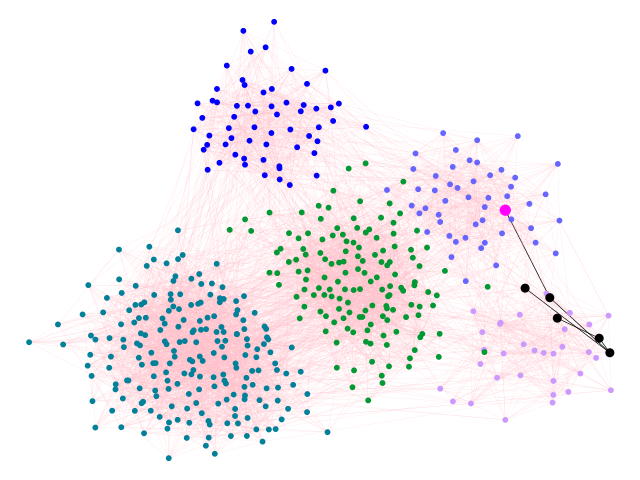
\includegraphics[width=0.80\linewidth]{images/network-1seed.png}
\caption{500 nodes, 1 seed}
\end{figure}
\begin{figure}[H]
\centering
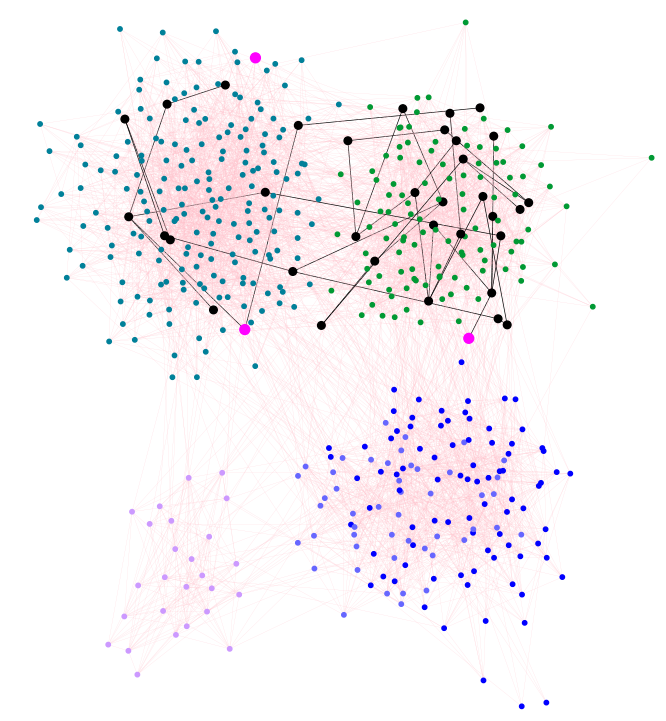
\includegraphics[width=0.80\linewidth]{images/netowrk-3seed.png}
\caption{500 nodes, 3 seeds}
\end{figure}
\begin{figure}[H]
\centering
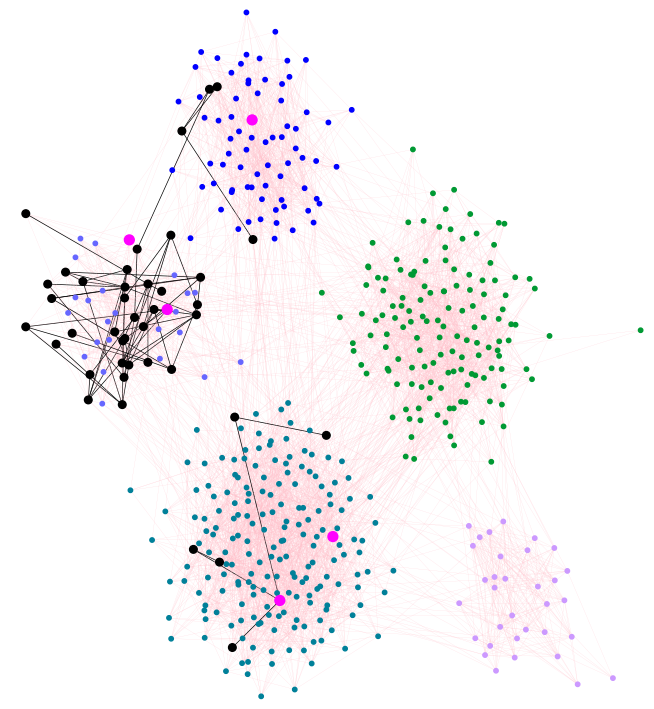
\includegraphics[width=0.80\linewidth]{images/network-5seed.png}
\caption{500 nodes, 5 seeds}
\end{figure}



\section{Components}
In the following, we present the four main components of our environment: the network, the advertisers, the auction and the publisher.


\subsection{Network}
Every node in the network has a category assigned at creation following a specified distribution of proportions. The edges are directional and every node has a number of outgoing edges drawn from a normal distribution with mean $2 * ln(number of nodes)$ and standard deviation $ln(number of nodes)$. This means that in a network of 1000 nodes an element will have $13.8\pm6.9$ outgoing connections. Outgoing connections have a chance to reach a node of the same category or one from a different category (the probability of cross category connections is specified in the settings). Nodes become seeds for an influence cascade when they interact with an advertisement, the influence propagates over the edges of the network which have an activation probability that depends on the categories on the nodes it connects: connections within a category group are the most likely to activate, those to an adjacent category group have a lesser change to activate and connections to a non adjacent category are the least likely to activate.


\subsection{Advertisers}

\begin{figure}[H]
    \centering
    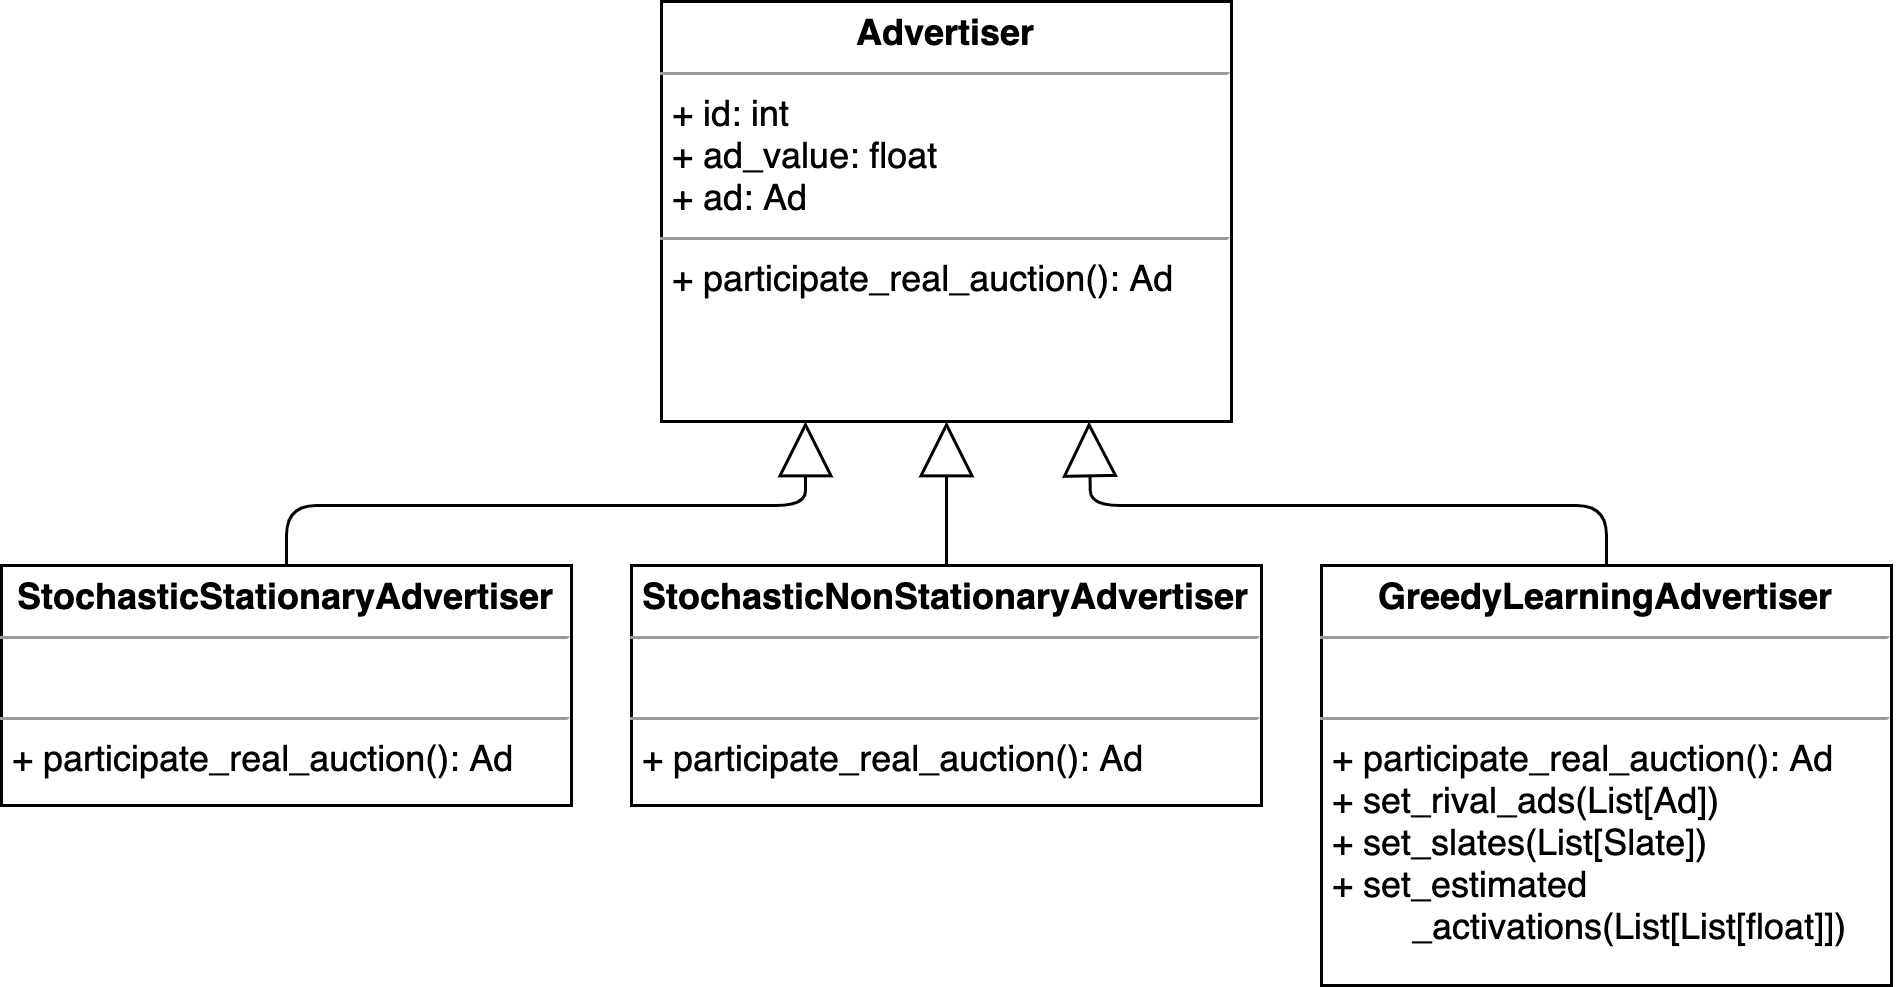
\includegraphics[width=0.66\linewidth]{images/advertisers-uml.png}
    \caption{Advertisers' classes.}
    \label{fig:vadvertisers-uml}
\end{figure}

We created a base Advertiser class that can participate to an auction. When the auction class calls the function \emph{participate\_real\_auction()}, it returns an Ad. The Ad contains the ID, its quality (different for each category), its value and the bid for each category.
Three classes are based on this advertiser.

\emph{StochasticNonStationaryAdvertiser} and \emph{StochasticStationaryAdvertiser} are both advertisers that, upon creation, randomly generate a set of bids for the Ad. The non-stationary version simply changes its ad and bids every n iterations.

The \emph{GreedyLearningAdvertiser} is the most complex class: when participate\_real\_auction is called, it starts the process of finding the optimal bids through simulations. It starts the simulation by not bidding anything for any category, then tries to increase the bid for each category separately and notes the gain.
It then calculates the marginal gain for each category as the current gain minus the gain in the preceding step, takes the maximum marginal gain and permanently set the bid in the corresponding category to the increased bidding level.
If all marginal gains are negative, it means that no immediate improvement is possible; the advertiser has found optimal bids, these are likely a local maximum.

Since it simulates the network, we assume that the advertiser knows the shape of the network, the activation probabilities and the quality of its ad. Moreover, we assume that it knows the other advertisers and their respective ads. After implementing this behaviour we drop some of these assumptions one by one.

\subsection{Auction}\label{subchap:Auction}
The job of the auction is to assign ads to all the slots available, these ads are then shown to the final user. In our scenario we have the social network that shows ads in a single slate composed by 6 slots, this slate is viewed by the user when browsing the social network.
The interaction of the user with the slate is modeled using a cascading model, the user sees the first ad then they can either engage with it or move on to the next one.

The real auction is run by the social network itself as it acts as a publisher, but also a simulated auction is run by the Greedy Advertiser when simulating a bids placement.

To assign ads to the slots we need to find the allocation that maximizes the expected value for the publisher, that is:

\[argmax_{s(a)} \{\sum_{a}\Lambda_{s(a)}{q_a}{b_a}\}\]

Where $s(a)$ is the slot assigned to the ad $a$, $\Lambda_{s(a)}$ is the slot's observation probability, $q_a$ is the quality of the ad (the probability that the user clicks the ad) and finally $b_a$ is the bid of the ad $a$.

Practically to find the allocation we simply sort the ads by decreasing order of $q_a*b_a$ and slots by decreasing order of observation probability, then we can assign to the first ad the first slot, to the second ad the second slot and so on.

The social network uses a cost-per-click model as a payment scheme so the auction also need to computer the price per click for every ad. As requested by the project's specification we used a classical VCG approach:

\[ p_a = \frac{1}{\Lambda_{s(a)}q_a}(X_a - Y_a) \]
\[ X_a = \max_{s(a')} \sum_{a'\neq a} \Lambda_{s(a')}q_{a'}v_{a'} \]
\[ Y_a = \sum_{a' \neq a} \Lambda_{\Bar{s}(a')}q_{a'}v_{a'} \]
\[ \Bar{s}(a') = arg\max_{s(a')} \sum_{a'} \Lambda_{s(a')}q_{a'}v_{a'} \]

Here we are calculating the price $p_a$ of ad $a$ using $X_a$ and $Y_a$. Note that each ad is assigned to at most one slot. $X_a$ is basically the total reward that other ads produce to the publisher if ad $a$ does not exist. While $Y_a$ is the total reward that other ads (different than ad $a$) produce to the publisher if ad $a$ exists. 
The pseudo-code for computing the price is the following:

\begin{algorithm}[H]
    \KwData{slate and available ads}
    \KwResult{Price for each ad in the slate}
    \For{slot in slate}{
        $a$ = ad assigned to the slot\;
        $ads\_except\_a$ = all available ads without ad $a$\;
        $allocation\_x\_a$ = compute the best allocation using $ads\_except\_a$\;
        $X_a$ = reward of the publisher using $allocation\_x\_a$\;
        
        $allocation\_y\_a$ = compute the best allocation using all ads\;
        $Y_a$ = reward of the publisher using $allocation\_y\_a$ but excluding the reward provided by ad $a$\;
    }
    \caption{Pseudocode for calculating the price of a click.}
\end{algorithm}


\subsection{Publisher}
The role of the publisher is to publish the ads to the network, it also provides the data that the advertisers need to execute simulations for calculating their bids. When required, the publisher uses bandit algorithms to estimate the values of ad qualities or the activation probabilities. When learning the values of ad qualities the publisher instantiates one bandit for every ad for every category, so if we have $7$ advertisers and $5$ categories there will be $35$ bandits, each with a number of arms that can be specified in the settings. The greater the number of arms the more precise our estimate will be, but it will also be harder to learn. At every step the current estimates are gathered with $get\_bandit\_qualities()$ and written into the ads. Then the episode is performed and feedback is collected which allows to calculate a sample estimate of the quality values and compare them to the bandit estimates. A reward of $1$ is assigned if the error between these two values is under a specified threshold otherwise the reward is $0$. The stochasticity of the reward is given by the fact that the sample estimate comes from a specific network realization. Estimating activation probabilities works in a very similar way: a bandit is created for every possible pair of categories so $25$ bandits if we have $5$ categories and environment feedback is used to assign rewards.


\subsection{Bandit Algorithms}

\subsubsection{UCB1}
In the UCB1 algorithm we associate to every arm an upper confidence bound. This upper confidence bound is created by summing the empirical mean and the confidence. At each round we pick the arm with the highest upper confidence and then update the empirical mean and the confidence with the obtained reward.

\subsubsection{Thompson Sampling}
In the Thompson Sampling algorithm we associate to each arm the parameters of a Beta distribution. At each round we draw a sample from the Beta distribution and choose the arm with the highest sample. Then with the obtained reward we update the beta parameters of the pulled arm.

\subsubsection{Sliding Window UCB1}
The behaviour of the Sliding Window UCB1 algorithm is pretty much similar to the one of the UCB1 except that the empirical mean and the confidence associated to every arm is calculated only on a subset of the rewards obtained. This subset of rewards with their respective pulled arms is composed of the latest $N$ results obtained, where $N$ is the length of the sliding window.

\subsubsection{Sliding Window Thompson Sampling}
Similarly the Sliding Window Thompson Sampling must only work with the latest $N$ samples, so each time a new reward is reported in a round we re-compute the Beta parameters for all arms using all the latest $N$ samples.
The computation of the Beta parameters is performed for all arms because the sample that is exiting the sliding window could be of any arm.



\section{Project development}
In this section we describe the project solution point by point.


\subsection{Social influence estimation}
Given a set of bids we can execute an auction and obtain the positioning of the ads in the slates given their qualities and bids. An auction is executed for every category of node since the same bid applies to all the nodes within a category. Given the slates with assigned ads we can use Monte Carlo estimation to evaluate the number of seeds and activated nodes generated by the campaigns. To calculate the seeds we model the interaction between the users and the ads. A user looks at the first ad in the slate for his category and a random sample is drawn, if this sample is smaller than the activation probability $p = ad  quality * slot  visibility$ then the node clicks the ad and becomes a seed, otherwise they move on to look at the second slot and so on while there are still ads in the slate. If a user clicks on an ad and becomes a seed, he stops looking at the ads that follow. Once a set of seeds is available we generate a live edge graph by drawing a sample for every edge in the network. The nodes activated by the seeds are calculated by walking the live edge graph. For every node we can also calculate the probability of being activated by the cascade. We examine the accuracy of the estimates as a function of the number of iterations in the Monte Carlo simulation. The error is the difference in the estimated node activation probability w.r.t. the baseline given by the best performing simulation.

\begin{figure}[H]
    \centering
    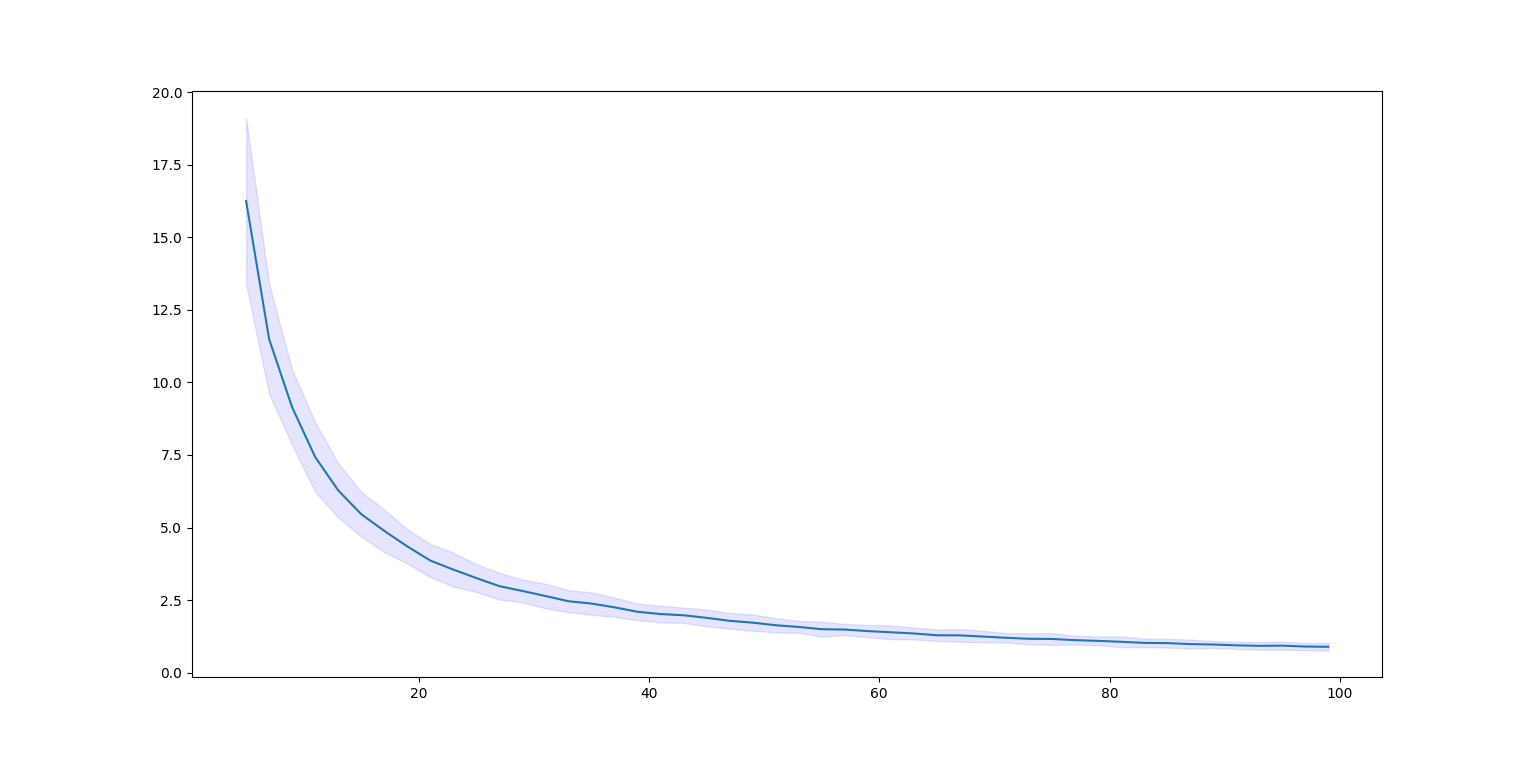
\includegraphics[width = \textwidth]{images/500 nodes step 2 50 tests each.png}
    \caption{Total error on node activation probability $\pm 2$ standard deviations against the number on MC iterations in a network of 500 nodes with 1000 iterations as baseline.}
\end{figure}

From theory we know that the number of iterations required to guarantee an error $\epsilon$ with a confidence bound $1-\delta$ is $R = O(\frac{1}{\epsilon^2}log(|S|)log(\frac{1}{\delta}))$. Given this we also expect the error to decrease logarithmically as the number of iterations increases which is confirmed by our experiment.
\newline

We can also analyze directly the number of nodes activated by the set of bids: in Figure \ref{fig:step1-1} is reported as an example the result of a single experiment run with different values of Monte Carlo iterations on a network of 100 nodes with only stationary stochastic advertisers.

\begin{figure}[H]
    \centering
    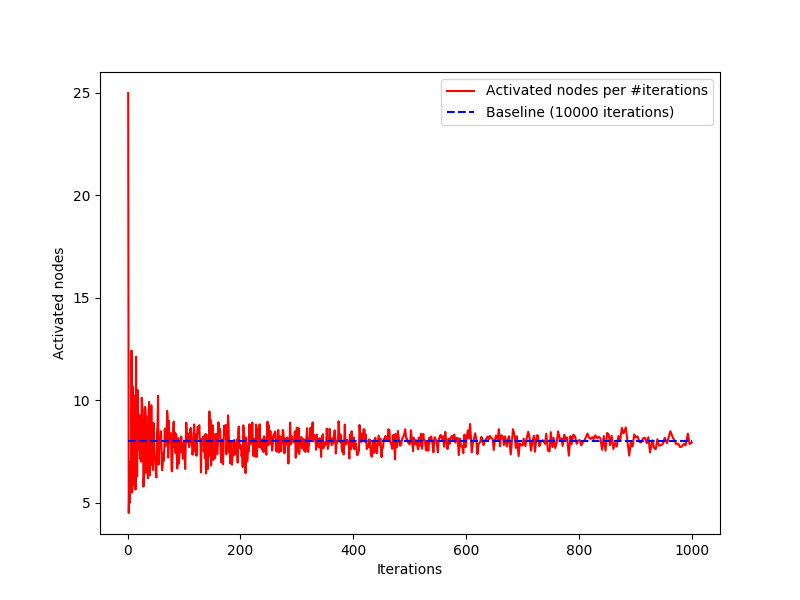
\includegraphics[width=0.66\linewidth]{images/step1-1-100nodes.png}
    \caption{Activated nodes per value of iterations}
    \label{fig:step1-1}
\end{figure}

While on Figure \ref{fig:step1-2} it is plotted the average performance gap of activated nodes on 20 experiments, performance gap interpreted as the absolute value of the difference between the baseline (in this case a Monte Carlo execution with 10'000 iterations) and the value returned by the execution.

\begin{figure}[H]
    \centering
    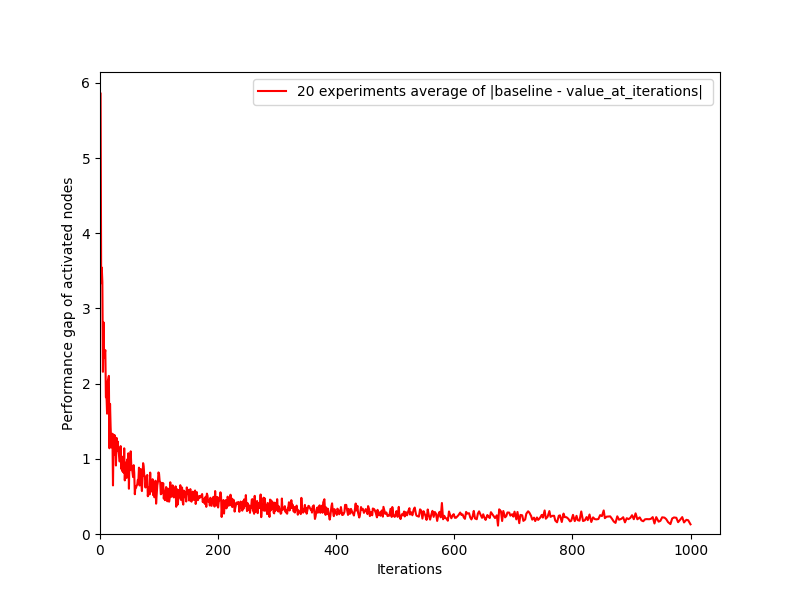
\includegraphics[width=0.66\linewidth]{images/step1-2-100nodes.png}
    \caption{Average error on 20 experiments per value of iterations}
    \label{fig:step1-2}
\end{figure}


\subsection{Problem formulation}
The problem that we need to solve is to find a bid for each category in order to maximize the difference between the expected gain and the expected cost: 
$$Gain = Revenue - Cost$$
The gain of a campaign (or a category) is given, in expectation, by the amount of nodes that activate in the network times the value of the activation $v_c$, while the cost is the price-per-click $p_c$ times the number of seeds (the advertiser pays only for the seeds): 
$$G_c = v_c E[activation]_c - p_cE[seeds]_c$$
Since the number of activation and seeds (in expectation) and the price-per-click depends to the position of the ad in the slate, they are a function of the bid used for that campaign. To have the highest gain we need to solve the following maximization problem:
$$G_c = \max_{b_c} v_cE[activation(b_c)]_c - p_c(b_c)E[seeds(b_c)]_c$$

It is possible to write the expected number of seeds as the sum over nodes that clicked the ad, where clicking the ad can be modeled as a random variable from a Bernoulli event:

\[E[seeds(b_c)]_c = \sum_{n=1}^{N}s_{n,c}(b_c)C_{n,c}\]
\[ s_{i,j}(b_c) \sim Bernoulli(\lambda(b_c)) \]

The parameter $C_{i,j}$ is a mask of value 1 if node i belongs to category j, 0 otherwise. It is necessary because the nodes can be seed only for their own category.
The parameter $\lambda_c$ depends on the position of the ad in the slate, and so on the bid. The slate is build in decreasing order of the quality times the value of each campaign ($q_cv_c$). So, we have that $\lambda_c$ is such that:

\[\lambda_c = \prod_{a \in \Bar{A_j}}\Lambda_{s(a)}q_a\]
\[\Bar{A_j} = \{a \in A \vert q_av_a \geq q_cv_c \}\]

This is a slightly pessimistic formulation since it assume that if the ad has the same quality times value of another advertiser campaign, it will be placed after him in the slate. Since the disposition in the slate is decided by the auctioneer, and the value of a campaign is a private information of the advertiser, the position in the slate and so the parameter $\lambda_c$ is usually estimated using the bids in replace of the values.
\newline

The price per click of each advertiser ($p_a$) for each campaign ($p_{a,c}$) is determined by the VCG auction (as presented in \autoref{subchap:Auction}) where, for the same reasons of parameter $\lambda_c$, the bids are often used instead of the value. 
With an abuse of notation, we referred to the price of the advertiser of the optimization problem as $p_c$ instead of $p_{\Bar{a},c}$.
\newline
If we assume that the 5 advertising campaigns are independent, the bids and the expected number of activation and seeds will be independent among different categories, and so the sum of the maximization of the five marginal gain will be equal to the maximization of the sum.
\newline
By introducing all these considerations in our formulation, we obtain the following optimization problem:
\[
G = \max_{b=[b_1,..b_K]} \sum_{c=1}^{K} v_cE[activation(b_c)]_c - \sum_{n=1}^{N}p_c s_{n,c} C_{n,c}
\]
\centerline{subject to:}
\[
\lambda_c = \prod_{a \in \Bar{A_j}}\Lambda_{s(a)}q_a
\]
\[ p_a = \frac{1}{\Lambda_{s(a)}q_a}(X_a - Y_a) \]
\[ X_a = \max_{s(a')} \sum_{a'\neq a} \Lambda_{s(a')}q_{a'}v_{a'} \]
\[ Y_a = \sum_{a' \neq a} \Lambda_{\Bar{s}(a')}q_{a'}v_{a'} \]
\[ \Bar{s}(a') = arg\max_{s(a')} \sum_{a'} \Lambda_{s(a')}q_{a'}v_{a'} \]

The only parameter that we did not define is the expected number of activated nodes given a set of bids. This is a parameter that depends on the expected number of seeds, but have also many dependence on the intrinsic parameters of the problem: number of nodes, connectivity, edges weight, categories distributions, and many other. 
Because of that, providing a mathematical distribution is an hard problem. A possible first approximation can be computed as a Gaussian distribution of mean and variance computed empirically over some simulation of the environment.


\subsection{Bidding with a greedy algorithm}
For this step, some \emph{stochastic\_advertisers} and one \emph{greedy\_learning\_advertiser} are created.
We give to the \emph{greedy\_advertiser} the information about its rivals and the slates, and then we ask it to participate to one auction.
The \emph{greedy\_advertiser} runs its simulation as described in Chapter 2.2, and stops when it reaches the first local optimum. 
The greedy learning will be influenced by the randomness of the simulation: a non-optimal set of bid can provide a a gain bigger than the expectation in some luckier run, that will result in all negative marginal gain in the next step and thus in the selection of a non-optimal bidding set.
From the data collected in a simulation we can plot the gain and the marginal gain for each improvement step (Figure \ref{fig:greedy_marginal_gain} and Figure \ref{fig:greedy_total_gain}). Note that the gain increases monotonically by definition since we stop the process when marginal gains are negative.

\begin{figure}[H]
\begin{minipage}{0.48\textwidth}
\centering
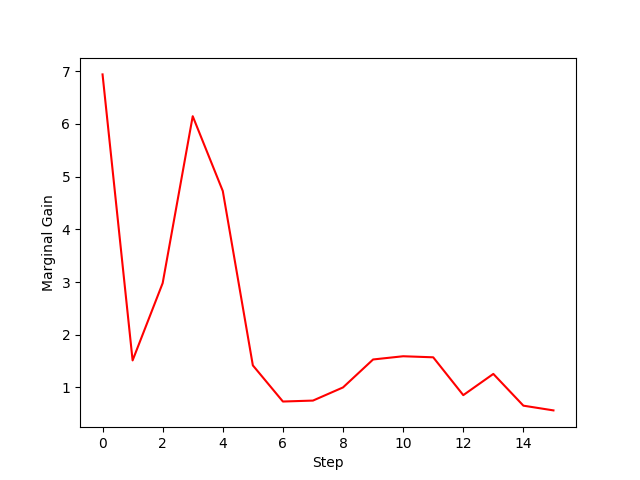
\includegraphics[width=1\linewidth]{images/step3-1.png}
\caption{Marginal gain of an example run}
\label{fig:greedy_marginal_gain}
\end{minipage}
\begin{minipage}{0.48\textwidth}

\centering
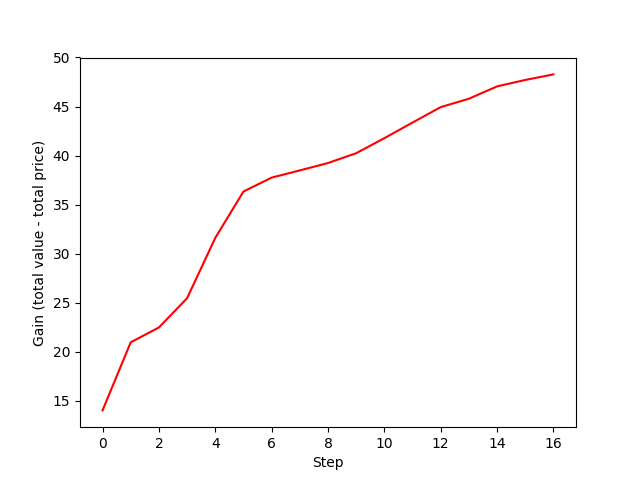
\includegraphics[width=1\linewidth]{images/step3-2.png}
\caption{Total gain of an example run}
\label{fig:greedy_total_gain}
\end{minipage}
\end{figure}

As reported in Chapter 3.2 the gain is the difference between the revenue and the cost for the advertiser. We can plot these two values separately to gain more insight on the improvement of the Greedy Advertiser: as can be seen in Figure \ref{fig:step3-3}. The Greedy advertiser starts by bidding a very small value for a single category so of course it will have a small price. Since it also bids a very low value it will obtain a slot that is one of the less observed, it follows that it will also obtain not many nodes' activations. Then, as soon as the Greedy Advertiser starts bidding more, it will of course pay more but also obtain a bigger revenue.

\begin{figure}[H]
    \centering
    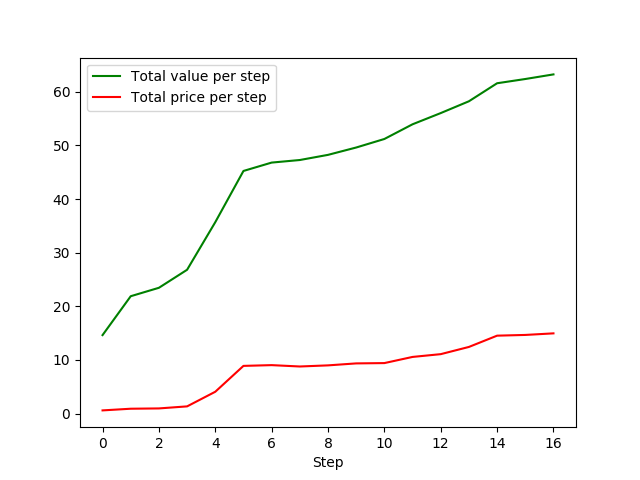
\includegraphics[width=0.66\linewidth]{images/step3-3.png}
    \caption{Revenue and cost for the advertiser in an example run}
    \label{fig:step3-3}
\end{figure}


\subsection{Online bid learning with unknown qualities and click probabilities}
In this step, we work in a situation in which the greedy learner does not know the qualities (and therefore the click probabilities) of the ads. 
In a VCG auction the position in the slate of an advertiser is determined by the product of the bid times the quality. Nodes also can be seeds only for one advertising campaign, therefore the position occupied in the slate can determine how much data we will be able to gather for learning our unknown parameters. The position in the slate also determines the cost per click that will be charged to the advertiser.
Since in a real situation the auctioneer do not know itself the real quality of the advertisement, the auction that he will perform will also be done using the estimation of the quality. This will generate different auction than the once produced in the ideal scenario, but more accurate with respect to a real word environment.
\newline
We apply bandit algorithms to solve the problem, and in the following we analyze the results and the differences among different techniques.
Considering that the arms of the bandit algorithm are a discretization of the possible qualities (in [0,1]), as reward of the pulled arm we used the following formula: 

\[ reward = \begin{cases} 
      1 & $if $ \vert pulled$ $quality - sampled$ $quality \vert  <= margin \\
      0 & $if $ \vert pulled$ $quality - sampled$ $quality \vert  > margin
\end{cases} \]

where with sampled quality we mean the empirical quality estimation obtained in a single day. The click probability is the product between quality and visibility so the measured quality is $\frac{seeds}{susceptible  Nodes} * 1 / visibility$. The margin is the distance between two arms.

We analyzed the problem using both UCB1 and Thompson Sampling, both in the case where only the first slot in the slate provides us information about the quality, and in the case where all the slots provided knowledge by considering the cascading model.
In the first case we will learn only the qualities associated to the ad winning the campaign (earning the first slot). Remembering that the real auction performed by the publisher is done with the estimated qualities, the first advertiser in the slate may sometimes not be the more proficient in terms of $quality*bid$, and so the learning may collect less data, especially in the first steps (as can be seen in Figure \ref{fig:first_only_ucb1} and Figure \ref{fig:first_only_ts})

\begin{figure}[H]

\begin{minipage}{0.48\textwidth}
\centering
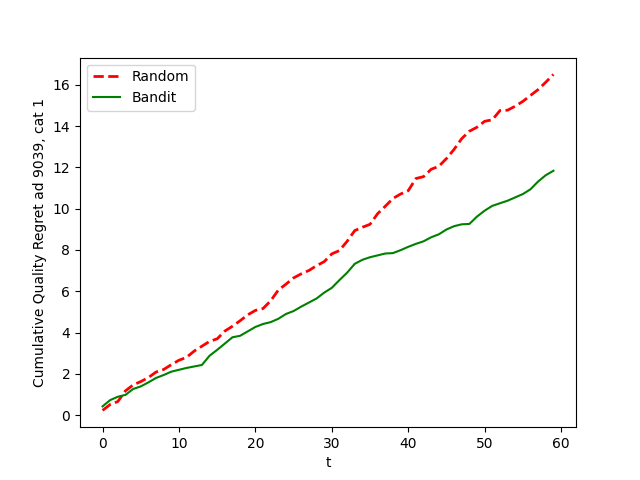
\includegraphics[width=1\linewidth]{images/first only ucb1.png}
\caption{Quality regret with UCB1 and first slot only}
\label{fig:first_only_ucb1}
\end{minipage}
\hfill
\begin{minipage}{0.48\textwidth}
\centering
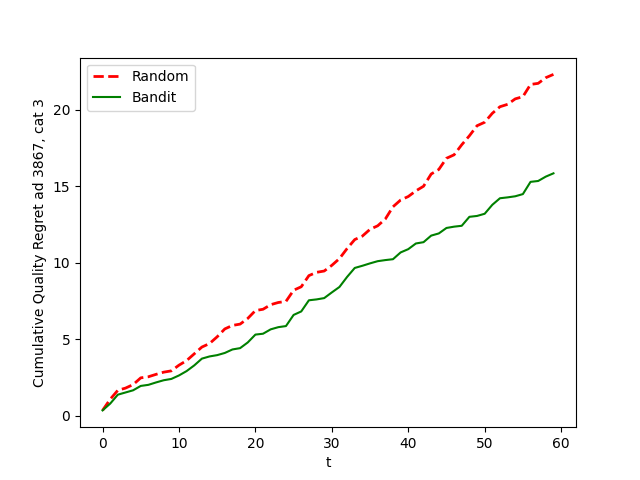
\includegraphics[width=1\linewidth]{images/First only ts.png}
\caption{Quality regret with Thompson Sampling and first slot only}
\label{fig:first_only_ts}
\end{minipage}

\end{figure}

In this two pictures, coming from two runs of 100 days, we can see how the use of only the first slate will lead to a slower learning. To improve the situation, we moved to the second scenario, where we used a cascading bandit algorithm to learn also from the advertiser not in the first position. To do that, we used the very same reward presented before, redefining only the sampled quality: to consider the position in the slate, in fact, the empirical reward is the ratio between the number of seeds for the advertiser and the total number of seeds that did not click on a previous ad (since we assume that any user will click on a single ad), multiplying by the prominence of the slot. Not considering the prominence would be equivalent to learning the product of the quality times the prominence, but this can not be done since the prominence is dependent to the position in the slate, and in principle could be different for each day. Finally, we discarded the data associated with ads with a number of susceptible seeds lower than the number of arms, since they suffered of too high bias.

In the following, we can see the results of the UCB1 and Thompson Sampling in this scenario.

\begin{figure}[H]

\begin{minipage}{0.48\textwidth}
\centering
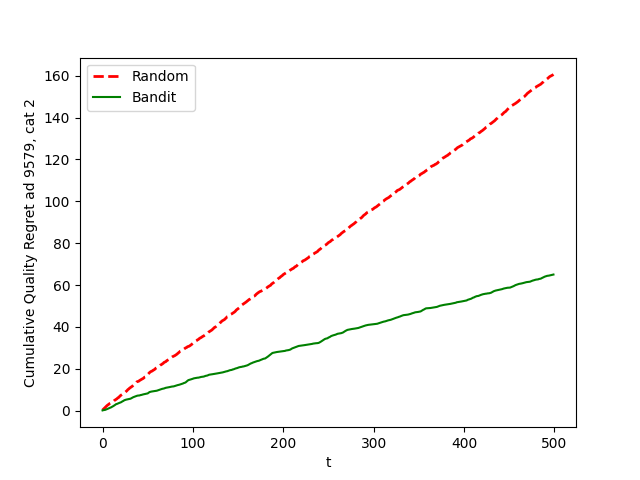
\includegraphics[width=1\linewidth]{images/quality UCB1 15 arm 500 nodes 500 days 5 iterations.png}
\caption{Quality cumulative regret with UCB1}
\end{minipage}
\hfill
\begin{minipage}{0.48\textwidth}
\centering
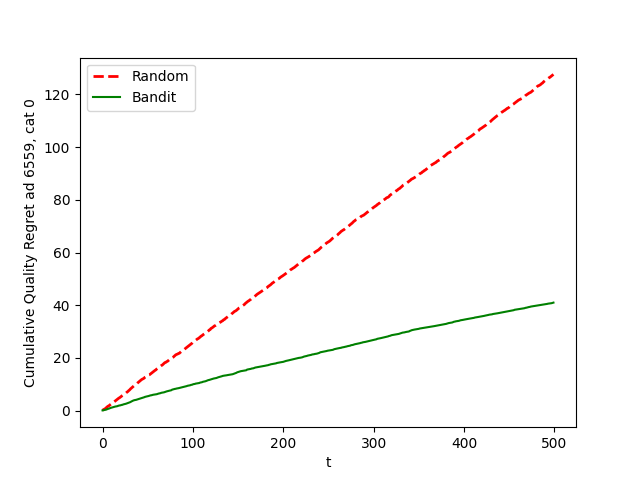
\includegraphics[width=1\linewidth]{images/quality TS 15 arm 500 nodes 500 days 5 iterations.png}
\caption{Quality cumulative regret with TS}
\end{minipage}

\end{figure}

It is also interesting to compare the performance of the bandits as the number of arms varies. From theory we expect to have faster learning with fewer arms but better optimums with more arms.
In the figures reported below we compare the cumulative regret obtained in scenarios with different number of arms.
\begin{figure}[H]
\begin{minipage}{0.33\textwidth}
\centering
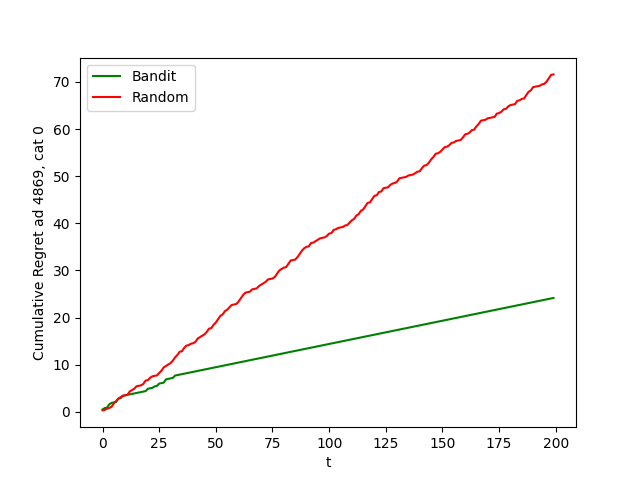
\includegraphics[width=1\linewidth]{images/quality 5 arms 200 days.png}
\caption{5 arms}
\end{minipage}
\begin{minipage}{0.33\textwidth}
\centering
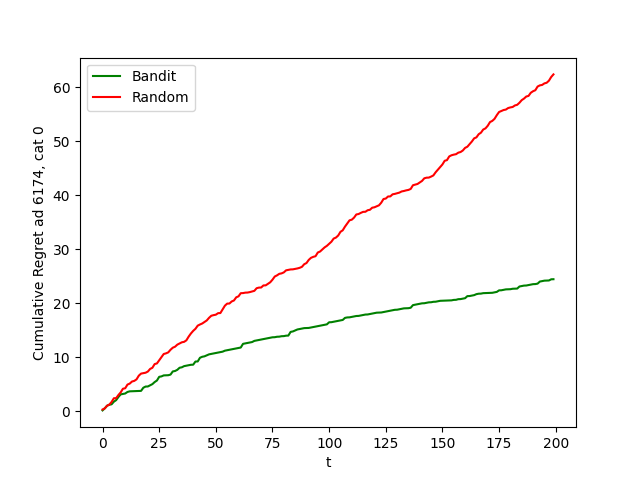
\includegraphics[width=1\linewidth]{images/quality 10 arms 200 days.png}
\caption{10 arms}
\end{minipage}
\begin{minipage}{0.33\textwidth}
\centering
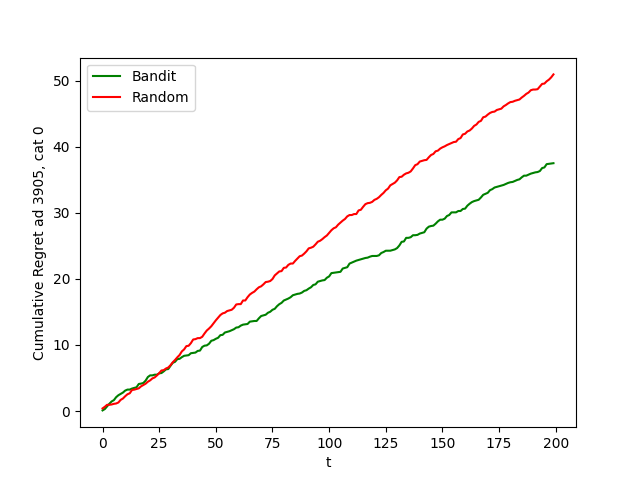
\includegraphics[width=1\linewidth]{images/quality 20 arms 200 days.png}
\caption{20 arms}
\end{minipage}
\end{figure}
We notice how with increasing number of arms it becomes harder to learn. However, given enough data, we can converge to an overall better solution as can be seen in Figure \ref{fig:step5_3000days}
\begin{figure}[H]
    \centering
    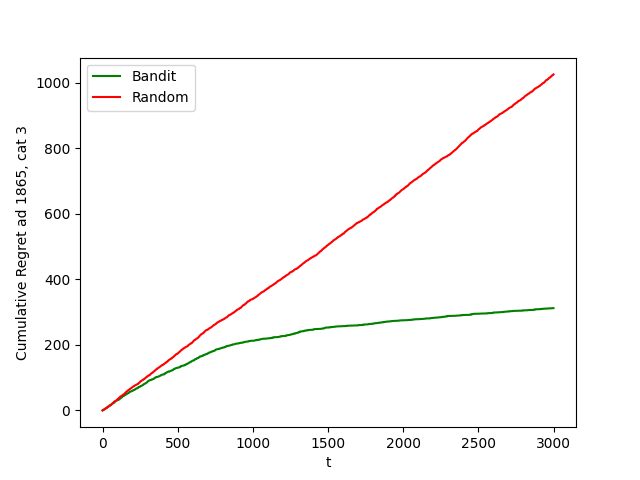
\includegraphics[width=0.66\linewidth]{images/quality 50 arms.png}
    \caption{Cumulative regret with 50 arms (3000 days)}
    \label{fig:step5_3000days}
\end{figure}

In this step we are also able to test the greedy advertiser performance versus the stochastic advertisers. As expected, the greedy advertiser shows a cumulative gain greater than the stochastic ones.

\begin{figure}[H]
    \centering
    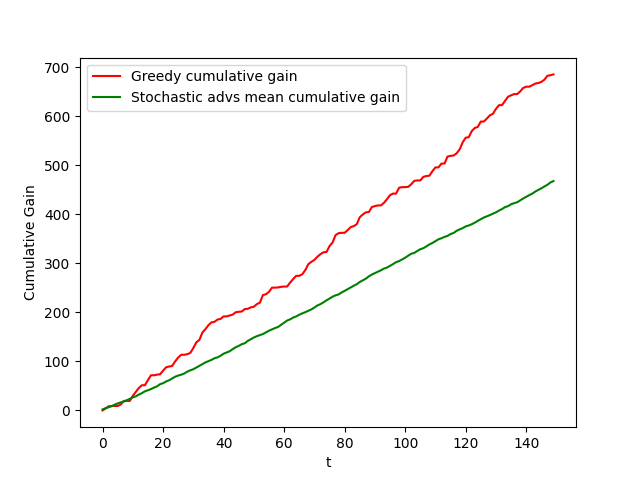
\includegraphics[width=0.55\linewidth]{images/greedy-vs-stochastics.png}
    \caption{Cumulative gain of advertisers.}
\end{figure}

\subsection{Online bid learning with unknown qualities, click probabilities and activation probabilities}

The task of learning the activation probabilities is similar to the one faced in the previous step to learn the qualities. Also in this case the knowledge of the activation probabilities affect the greedy learning procedure, since it directly determines the accuracy of the simulation and, as consequences, the estimation of the gain by the learner.
In this case the arms are the discretization of the possible activation probabilities, but in the range of [0, max\_probability]: this is done because the maximum value of the activation probability is much lower than 1, and so it allow us to instantiate more arms in useful positions and be more precise in the learning. The reward is, instead, computed as follows:
\[ reward = \begin{cases} 
      1 & $if $ \vert pulled$ $activation - sampled$ $activation \vert  <= margin \\
      0 & $if $ \vert pulled$ $activation - sampled$ $activation \vert  > margin
\end{cases} \]
where the sampled activation is the ratio of the edges between the two categories in question which activated in the episode.

In the figure below it is possible to see the cumulative regret of the Thompson Sampling algorithm applied to the value of the activation probability for edges between nodes of the first category (same analysis can be done for UCB1 algorithm).

\begin{figure}[H]
    \centering
    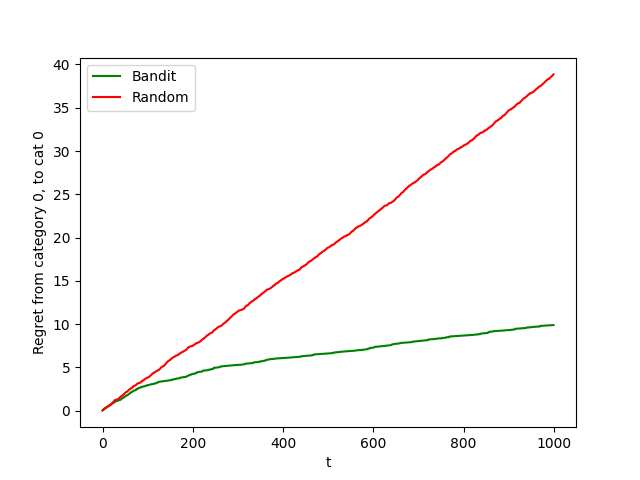
\includegraphics[width=0.66\linewidth]{images/activation 20 arms.png}
    \caption{Cumulative regret for 20 armed bandit estimating the activation probability}
\end{figure}


\subsection{Online bid learning with unknown qualities, click probabilities and activation probabilities, in the context of non stationary advertisers}
In a non stationary context the adversaries change their ads and bids periodically therefore we need to adapt our optimization process. This is done by using sliding windows on the rewards for the estimation of the qualities. The size of the sliding window has to be large enough to contain enough samples for learning the target values and small enough to discard old values as soon as possible. We use the cumulative regret to evaluate the performance of this method using both Sliding Window Thompson Sampling and Sliding Window UCB1. We obtain from them a very similar result where we can notice that the bandit after the abrupt change reaches a new optimum as soon as many old sample have been discarded.

\begin{figure}[H]

\begin{minipage}{0.48\textwidth}
\centering
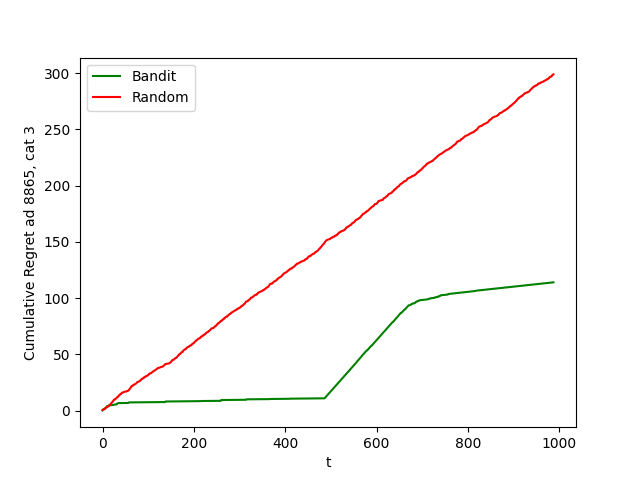
\includegraphics[width=1\linewidth]{images/quality sliding window.png}
\caption{Sliding Window Thompson Sampling; abrupt change at t=500; sliding window size=250; bandit with 10 arms.}
\end{minipage}
\hfill
\begin{minipage}{0.48\textwidth}
\centering
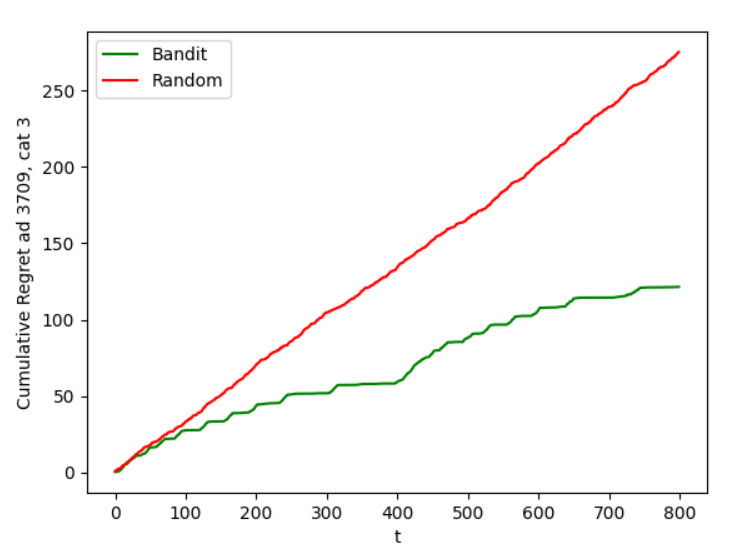
\includegraphics[width=1\linewidth]{images/sliding window ucb.png}
\caption{Sliding Window UCB1; sliding window size=400; bandit with 10 arms.}
\end{minipage}

\end{figure}



\section{Analysis of the results}
The first part of our project consisted in creating a model of the network and executing Monte Carlo simulations on it. We made use of specialised data structures in order to speed up the execution, for example a list of active edges along with the adjacency matrix. We chose the parameters of the network such as edge activation probabilities and click probabilities in a way to have reasonable cascades. We tried to avoid situations in which just one seed always activates the entire network and those in which it is extremely hard to activate any node at all.

The greedy learning advertiser always performs better than the stochastic advertisers in a sufficient amount of time, however it doesn't normally find the global optimal solution.

When we drop the assumption of knowing some data we notice a decrease in performance, as expected, this is due to the fact that the solution is calculated by simulating the network and the accuracy of the simulation determines the precision of the solution. For this reason we reach the optimal solution later, after learning the correct estimation.

In our experiments we confirm some expected results from theory, for example the dependency between learning performance and the number of arms and the number of samples. When we are allowed to gather data for ads only when they are in the first position in a slate we expect to learn much less, because we will have less data since most ads will not be in the first position most of the time.

\newpage
\appendix

\section{Code technicalities}

The runnable scripts used to run analyses and create plots are $step1.py$, $step3.py$ and $step4\_5\_6.py$. Each script comes with a first section called "Constants" that includes variables which are used as settings for that particular analysis.

There are also global settings that are stored in the variables contained in $constants.py$, for example there are stored the number of nodes in the network, the number of categories, the number of slots in a slate and many others global variables.
\newline

Also, there are runnable scripts in the $tests$ folder that are used internally to check the correctness of the algorithms. For example the script $test\_vcg\_auction.py$ contains some unit tests to check the correctness of the VCG Auction code.

\end{document}